
% !TeX program = lualatex
% !TeX encoding = utf8
% !TeX spellcheck = uk_UA
% !BIB program = bibler

\documentclass{beamer}
\usetheme{Electromagnetism}
\usepackage{Electromagnetism}
\usetikzlibrary{spy}
\hypersetup{
  colorlinks=true,
  linkcolor=cyan,  % Цвет для внутренних ссылок
  urlcolor=red,    % Цвет для URL
  citecolor=blue   % Цвет для библиографических ссылок
}


%\def\colform#1{
%    \tikz[baseline]{\node[fill=green!50, rectangle, anchor=base, font=\scriptsize]{#1}}
%}


%============================================================================
\title[Лекції електрики та магнетизму]{\huge\bfseries Магнітне поле у речовині}
\subtitle{Лекції з електрики та магнетизму}
\author{Пономаренко С. М.}
\date{}
%============================================================================
\graphicspath{{pictures/}}

\begin{document}


\begin{frame}[plain]
	\maketitle
	%	\tikz[remember picture,overlay] \node[opacity=0.7,inner sep=0pt,
	%		anchor=north west] at (current page.north
	%	west){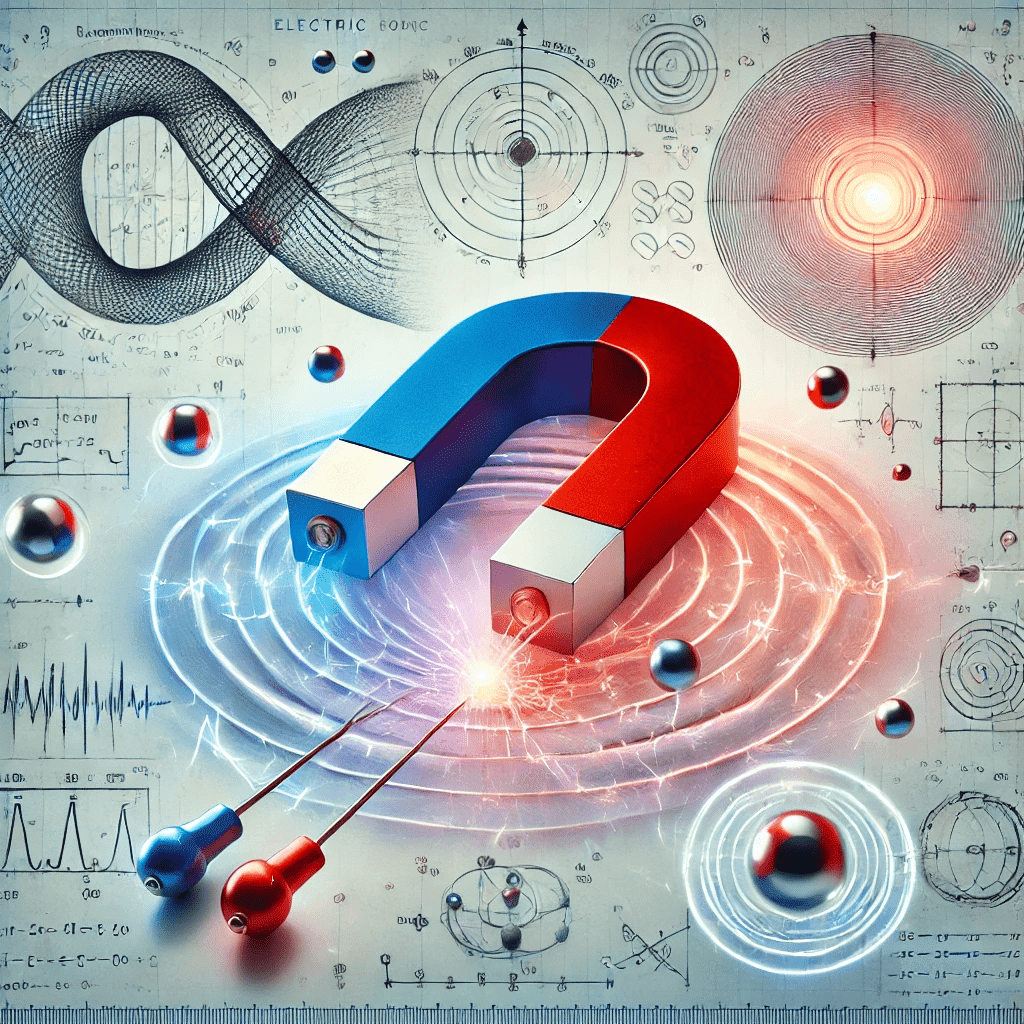
\includegraphics[width=2cm]{EMInteractions}};
\end{frame}

% ============================== Слайд ## ===================================
\begin{frame}{Зміст лекції}{}
	\tableofcontents
\end{frame}
% ===========================================================================


% ============================== Слайд ## ===================================
\begin{frame}{Гіпотеза Ампера}{Молекулярні струми}
	\begin{block}{}\justifying
		Якщо магнітне поле діє на рухомі заряджені частинки та рамки зі струмом, то \alert{чому воно також діє і на будь-який інший
			шматок магніту}? Ампер припустив, що \alert{всередині магніту теж течуть струми}.
	\end{block}


	\begin{block}{}\justifying\scriptsize
		Але якщо взяти стрілку або магніт у руки, то ніяких струмів ми не відчуваємо. Отже,  ці струми циркулюють усередині речовини і
		ніколи не виходять назовні. Що це за струми такі всередині речовини, Ампер звісно ж не знав. Сучасній науці вже відомо, що звичайна речовина
		складається з атомів. Своєю чергою, всередині атомів є позитивно заряджені ядра з негативно зарядженими електронами, що обертаються навколо них.
		Також самі електрони є маленькими магнітними стрілочками. Так
		ось, рух електронів усередині атомів є не що інше, як електричні струми, про існування яких припустив Ампер. Магнітне поле діє на ці струми, а
		значить і на речовину в цілому.
	\end{block}


	\begin{center}
		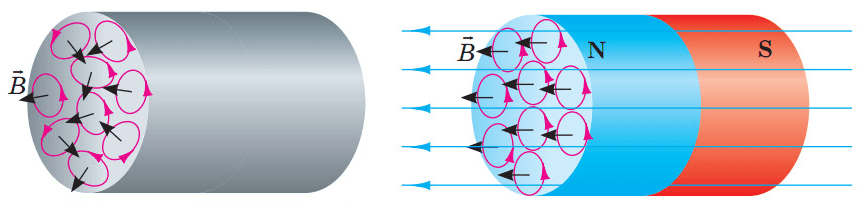
\includegraphics[width=1\linewidth]{AmpereHypotesis}
	\end{center}

\end{frame}
% ===========================================================================



% ============================== Слайд ## ===================================
\begin{frame}{Означення}{}
	\framesubtitle<1>{Мікрополе та середнє поле}
	\framesubtitle<2>{Струми провідності та молекулярні струми}
	\begin{onlyenv}<1>
		\begin{block}{}\justifying
			У речовині магнітне поле формується як зовнішнім полем, так і струмами, що циркулюють у цій речовині.

			\bigskip

			На мікрорівні (тобто на відстанях
			порядку розміру атомів і менше) поле різко змінюється в часі та просторі. Це поле називається \alert{мікрополем} $\Bfield_\text{micro}$ .
			Однак якщо провести усереднення за малим об'ємом, у якому є багато частинок (тобто за фізично нескінченно малим об'ємом), то отримаємо
			середнє поле:
			\begin{equation*}
				\left\langle \Bfield\right\rangle = \frac1{\Delta V} \iiint\limits_{\Delta V}
				\Bfield_\text{micro} dV.
			\end{equation*}
			\alert{Середнє поле} змінюється істотно повільніше внаслідок статистичного усереднення при випадковому русі частинок.
		\end{block}
	\end{onlyenv}
	\begin{onlyenv}<2>
		\begin{block}{}\justifying
			Створювані рухомими зарядами, можна розділити на дві групи: \alert{струми провідності} та \alert{молекулярні струми}.
			\begin{enumerate}
				\item \alert{Струми провідності} пов'язані з переміщенням вільних зарядів і є сторонніми щодо речовини.
				\item \alert{Молекулярні струми} зумовлені орбітальним рухом і спіном (власним моментом імпульсу) електронів в атомах (молекулах) і ядер речовини.
			\end{enumerate}
		\end{block}
	\end{onlyenv}
\end{frame}
% ===========================================================================


% ============================== Слайд ## ===================================
\begin{frame}{Вектор намагнічування}{}
	\begin{block}{}
		\alert{Вектор намагнічування} (або \alert{намагніченість}) — це величина, що характеризує магнітний момент одиниці об'єму речовини. Визначається вона
		як:

		\begin{equation*}
			\vect{J} = \frac{1}{V}\sum_i\vect{p}_i,
		\end{equation*}

		де $\vect{p}_i$ --- магнітні моменти окремих частинок.
	\end{block}


	\begin{block}{}\justifying\small
		Намагніченість називається \alert{однорідною}, якщо вектор $I$ не залежить від вибору точки в речовин. Якщо ж $\vect{I}\neq\const$, то намагніченість
		називається \alert{неоднорідною}.
	\end{block}
	\begin{center}
		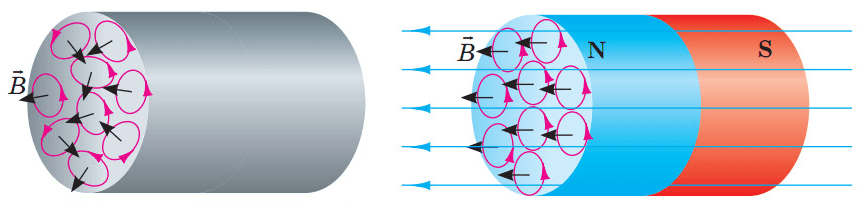
\includegraphics[width=1\linewidth]{AmpereHypotesis}
	\end{center}
\end{frame}
% ===========================================================================



% ============================== Слайд ## ===================================
\begin{frame}{Зв'язок намагніченості з молекулярними струмами}{}


	\begin{block}{}\justifying\scriptsize
		Виділимо в речовині досить малий циліндр, так що поле в ньому можна вважати практично однорідним. У його об'ємі молекулярні струми компенсують один
		одного. Циліндр (ліворуч) і вигляд його торця (праворуч). Кільцеві струми, що циркулюють в об'ємі, компенсують один одного всюди, окрім точок бічної
		поверхні. У результаті залишається тільки поверхневий струм, що тече бічною поверхнею циліндра.
	\end{block}
	\begin{columns}
		\begin{column}{0.5\linewidth}\centering
			\begin{tikzpicture}[>=latex]
				\draw[fill=gray!20] (0,0) arc(180:350:1 and 0.2) -- ++(45:2)  arc(350:180:1 and 0.2) -- cycle;
				                \path (45:2) ++(1,0) coordinate (O);

				\begin{scope}[shift={(O)}, yscale=0.2]
					\draw[thick, blue, arrowpos={0.7}{2pt}{3pt}] (0,0) [partial ellipse=0:360:1];
					\foreach \a in {10, 40,...,340} {
							\draw[red, smooth, arrowpos={0.75}{2pt}{3pt}] (\a:0.8) [partial ellipse=0:360:0.2];
						}
					\foreach \a in {25,85,...,335} {
							\draw[red, smooth] (\a:0.42) [partial ellipse=0:360:0.2];
						}
					\draw[red, smooth] (0, 0) [partial ellipse=0:360:0.2];
				\end{scope}

				\foreach \l in {0.2,0.4,...,1.8} {
						\draw[blue, arrowpos={0.4}{2pt}{3pt}] (45:\l) arc(180:350:1 and 0.2);
					}
				\draw[->, ultra thick] (O) -- ++(0,1) coordinate (J) node[left] {$\vect{J}$};
				\draw (0,0) -- ++(0,2);
				\draw (0,0) ++(0, 0.5) arc (90:45:0.5) node[pos=0.5, anchor=south] {$\theta$};
                \draw[->] (O) -- ++(45:{1*cos(45)}) coordinate (Pr) node[right] {$\ell\vect{\tau}$};
                \draw[dashed] (J) -- (Pr);
				\draw[<->] (2.2, 0) -- node[right] {$\ell$} ++(45:2);
			\end{tikzpicture}
		\end{column}
		\begin{column}{0.5\linewidth}\centering
			\begin{tikzpicture}[>=latex]
				\draw[arrowpos={0.4}{2pt}{4pt}, thick, blue] (0,0) [partial ellipse=0:360:1.01];
				\foreach \a in {10, 40,...,340} {
						\draw[arrowpos={\a/360}{2pt}{3pt}, red] (\a:0.8) [partial ellipse=0:360:0.2];
					}
				\foreach \a in {25,85,...,335} {
						\draw[arrowpos={\a/360}{2pt}{3pt}, red] (\a:0.42) [partial ellipse=0:360:0.2];
					}
				\draw[arrowpos={0.5}{2pt}{3pt}, red] (0, 0) [partial ellipse=0:360:0.2];
			\end{tikzpicture}
		\end{column}
	\end{columns}
\begin{block}{}
Знайдемо магнітний момент такого циліндрика:
    \begin{equation*}
    \vect{p}_m = \vect{J}V = \frac1c I_mS\ \vect{n} \Rightarrow\ \vect{J}S\ell\cos\theta = \frac1c I_m S\ \vect{n}
    \Rightarrow\ \vect{J}\cdot\vect{\ell} \ell\cos\theta  = \frac1c I_m \ \vect{n}\cdot\vect{\ell}
\end{equation*}
\begin{equation*}
    \frac{I_m}{\ell} = i_m = c\vect{J}\cdot\vect{\ell}.
\end{equation*}
\end{block}
\end{frame}
% ===========================================================================


\end{document}
